\documentclass[a4paper,12pt]{article}
\usepackage[utf8]{inputenc}
\usepackage{hyperref}
\usepackage{graphicx,float}
\graphicspath{{images/}}
\usepackage[T1]{fontenc}
\usepackage[polish]{babel}
\usepackage{lmodern}
\usepackage{amsmath}
\usepackage{xcolor}
\usepackage{listings}
\usepackage[top=2cm,bottom=3cm,left=3cm,right=3cm]{geometry}
\usepackage{titlesec}
\titlelabel{\thetitle.\hspace{0.3em}}

\lstset{
    language=C++,
    basicstyle=\ttfamily\footnotesize,
    inputencoding=utf8,
    extendedchars=true,
    literate={ą}{{\k{a}}}1 {Ą}{{\k{A}}}1
             {ć}{{\'{c}}}1 {Ć}{{\'{C}}}1
             {ę}{{\k{e}}}1 {Ę}{{\k{E}}}1
             {ł}{{\l}}1 {Ł}{{\L}}1
             {ń}{{\'{n}}}1 {Ń}{{\'{N}}}1
             {ó}{{\'{o}}}1 {Ó}{{\'{O}}}1
             {ś}{{\'{s}}}1 {Ś}{{\'{S}}}1
             {ż}{{\.{z}}}1 {Ż}{{\.{Z}}}1
             {ź}{{\'{z}}}1 {Ź}{{\'{Z}}}1,
    numbers=left,
    numberstyle=\tiny,
    stepnumber=1,
    numbersep=8pt,
    frame=single,
    framerule=0.4pt,
    framesep=3pt,
    breaklines=true,
    breakatwhitespace=false,
    columns=fullflexible,
    keepspaces=true,
    tabsize=4,
    showstringspaces=false,
    xleftmargin=2.2em,
    framexleftmargin=2.2em
}

\begin{document}
    \thispagestyle{empty}
    \vspace{1em}
    \noindent
    \begin{minipage}{0.48\textwidth}
        \raggedright
        Wydział: W4N\\Rok: 2025/2026\\Semestr: 5
    \end{minipage}
    \begin{minipage}{0.48\textwidth}
        \raggedleft
        Data oddania pracy:\\\today
    \end{minipage}
    \vspace{10em}
    \noindent
    \begin{center}
        \rule{\textwidth}{0.5pt}\\\vspace{2em}
        {\Huge\textbf{S}\Large\textbf{YSTEMY OPERACYJNE}}\\\vspace{1em}
        {\large\textbf{Projekt wielowątkowego serwera usług z obsługą priorytetów i kontrolą dostępu do zasobów}}\\\vspace{1em}
        \rule{\textwidth}{0.5pt}\\\vspace{4em}
        {\large Autor:}\\\vspace{0.5em}
        {\Large Kacper Piekut 280879}\\\vspace{3em}
        {\large Prowadzący:}\\\vspace{0.5em}
        {\Large dr Marek Bazan}
    \end{center}
    \vspace{6em}
    \begin{picture}(0,0)
        \put(0,-250){
\includegraphics[height=4cm]{logo pwr.png}}
    \end{picture}
    \newpage
    \vspace*{1em}
    \section{Wstęp}
        \vspace{1em}
        Współbieżność w systemach operacyjnych i aplikacjach serwerowych jest kluczowym zagadnieniem pozwalającym zwiększać przepustowość oraz skracać czasy odpowiedzi poprzez równoległe wykonywanie zadań. Jednocześnie wprowadza ona szereg wyzwań teoretycznych i praktycznych, takich jak warunki wyścigu (Race Conditions), zakleszczenia (Deadlocks), zagłodzenie (Starvation) czy zapewnienie spójności danych przy jednoczesnym dostępie wielu wątków. Rozwiązanie tych problemów wymaga stosowania odpowiednich prymitywów synchronizacji oraz świadomego projektowania architektury. Do najważniejszych mechanizmów synchronizacji należą blokady wzajemne (std::mutex) zapewniające wyłączny dostęp do sekcji krytycznych, blokady współdzielone (std::shared\_mutex) pozwalające wielu czytelnikom jednocześnie odczytywać zasób przy zachowaniu wyłączności dla pisarza, warunki (std::condition\_variable) umożliwiające efektywne oczekiwanie na zdarzenia. W praktyce serwerowej często stosuje się również pule wątków (Thread Pool), które pozwalają kontrolować liczbę aktywnych wątków i równomiernie rozdzielać pracę, oraz kolejki priorytetowe do porządkowania zadań według ważności.
        \vspace{2em}
    \section{Cele projektu}
        \vspace{1em}
        Celem projektu jest stworzenie i analiza wielowątkowego serwera usług w języku C++, który demonstruje poprawne i efektywne mechanizmy synchronizacji na dwóch poziomach - globalnym i lokalnym - oraz wpływ priorytetów zadań na działanie systemu. W szczególności:
        \begin{itemize}
            \item Zaprojektowanie architektury z kilkoma usługami współdzielącymi zasoby globalne.
            \item Implementacja lokalnego wzorca producent-konsument: każda usługa posiada własną kolejkę priorytetową zadań oraz pulę wątków roboczych.
            \item Implementacja ochrony zasobów globalnych zgodnie z modelem czytelnicy-pisarze - równoległe odczyty, wyłączny zapis.
            \item Zaimplementowanie mechanizmu łagodnego zamykania (graceful shutdown): po sygnale zatrzymania przestajemy przyjmować nowe zadania i kończymy dopiero po opróżnieniu kolejek.
            \item Weryfikacja spójności przez liczniki zadań (produced i done) oraz raport końcowy potwierdzający, że wszystkie zlecone zadania zostały przetworzone.
        \end{itemize}
    \newpage
    \vspace*{1em}
    \section{Plan eksperymentu}
        \vspace{1em}
        \textbf{Testowany system}\\
        \vspace{-0.5em}\\
        Przedmiotem badań jest wielowątkowy serwer usług napisany w języku C++. System składa się z wielu usług, z których każda posiada własną lokalną kolejkę priorytetową zadań oraz pulę wątków roboczych. Zasoby globalne są współdzielone i chronione odpowiednio za pomocą std::shared\_mutex (model czytelnicy-pisarz) oraz std::mutex.\\
        \vspace{0.5em}\\
        \textbf{Środowisko testowe}\\
        \vspace{-0.5em}\\
        Eksperyment jest wykonywany w środowisku konsolowym na systemie Windows. Kod kompilowany jest przy użyciu kompilatora MinGW (GCC) w wersji 13.2.0; uruchamianie odbywa się z poziomu konsoli systemu.\\
        \vspace{0.5em}\\
        \textbf{Specyfikacja sprzętowa}\\
        \vspace{-0.5em}\\
        Laptop: ASUS TUF Gaming F15.\\
        Procesor: Intel Core i5-11400H, 6 rdzeni, 12 wątków, taktowanie bazowe 2.7 GHz (do 4.5 GHz w trybie turbo).\\
        Pamięć RAM: 16 GB DDR4.\\
        Dysk: SSD NVMe 512 GB (Samsung MZVLQ512HBLU-00B00).\\
        Karta graficzna: NVIDIA GeForce RTX 3050 Laptop GPU\\oraz Intel UHD Graphics.\\
        System operacyjny: Microsoft Windows 11 Home 64-bit, wersja 10.0.26100.
    \newpage
    \vspace*{1em}
    \section{Implementacja}
        \vspace{1em}
        Poniżej przedstawiono szczegółowy opis implementacji programu, plik po pliku, wraz z omówieniem kluczowych klas, funkcji i zastosowanych mechanizmów synchronizacji.
        \vspace{1em}
        \subsection{Struktura projektu}
            \vspace{-0.2em}
            Projekt znajduje się w folderze głównym i składa się z następujących plików:
            \begin{itemize}
                \item main.cpp - punkt wejścia programu oraz miejsce konfiguracji przebiegu. Zawiera uruchomienie domyślne programu oraz tryb testowy z trzema scenariuszami, które modyfikują tylko parametry i logi, bez zmiany architektury usług.
                \item Task.hpp - definicja zadania (Task) oraz komparatora priorytetów (TaskCompare). Ten plik określa, jakie informacje niesie zadanie (id, priorytet, dane tekstowe) i w jaki sposób kolejka rozstrzyga kolejność obsługi.
                \item SafePriorityQueue.hpp - bezpieczna wątkowo kolejka priorytetowa oparta o std::priority\_queue. Odpowiada za synchronizację dostępu (mutex, condition\\\_variable) oraz mechanizm zamykania (close), który pozwala wątkom roboczym zakończyć pracę po opróżnieniu kolejki.
                \item SharedResources.hpp - wspólne zasoby używane przez wszystkie usługi. Zawiera Logger (z możliwością wyciszenia logów w testach) oraz DataPool chroniony blokadą współdzieloną w modelu czytelnicy-pisarz.
                \item Service.hpp / Service.cpp - implementacja pojedynczej usługi działającej jako producent-konsument. Klasa zarządza pulą wątków roboczych, lokalną kolejką zadań, licznikami produced/done oraz poprawnym startem i zatrzymaniem.
            \end{itemize}
        \newpage
        \vspace*{2em}
        \subsection{Plik main.cpp}
            \vspace{-0.2em}
            Punkt wejścia programu. Plik zawiera tryb uruchomienia domyślnego oraz tryb testowy (scenariusze), które wykorzystują ten sam przebieg programu, a różnią się jedynie parametrami i dodatkowymi logami:
            \begin{itemize}
                \item Zawiera flagę testMode, która decyduje czy program uruchamia się w trybie domyślnym, czy w trybie scenariuszy.
                \item Zawiera flagę terminalLogMode, która steruje wypisywaniem logów w terminalu (nie wpływa na zapisywanie logów do pliku).
                \item Na początku przygotowywana jest ścieżka do pliku logów: sprawdzany jest katalog logs (w razie potrzeby tworzony), a nazwa pliku ma format logs-dd-mm-rrrr\_gg-mm.txt (czas uruchomienia programu z dokładnością do minuty).
                \item Definiuje funkcję uruchamiającą przebieg programu (run\_default\_program), która tworzy SharedResources oraz dwie usługi: DataService (50 wątków) i ReportService (50 wątkow), a następnie uruchamia je metodą start().
                \item W pętli generuje określoną liczbę par zadań i przekazuje je do odpowiednich usług; stosowane jest krótkie opóźnienie sleep\_for(5 ms), aby zasymulować napływ pracy.
                \item Po zakończeniu generowania zadań program odczekuje określony czas (stopAfter), a następnie wywołuje stop() na obu usługach.
                \item Na koniec sumuje liczniki produced\_count() oraz done\_count() obu usług i wypisuje raport w konsoli w formie: Wygenerowane: X Wykonane: Y Status: OK/MISMATCH.
                \item Po zatrzymaniu usług bufor logów jest zapisywany do pliku w katalogu logs poprzez wywołanie metody dumpToFile na obiekcie logger.
                \item Tryb testowy: program pyta o numer scenariusza (1/2/3), a następnie ustawia parametry przebiegu.
                \item Scenariusz 1: wielokrotne uruchomienie tego samego przebiegu (np. 10 razy) z wyciszonymi logami (Logger wyłączony), aby sprawdzić spójność (oczekujemy X = Y).
                \item Scenariusz 2: w trakcie generowania zadań do kolejki DataService wstrzykiwane jest dodatkowe zadanie o bardzo wysokim priorytecie wraz z logiem informacyjnym.
                \item Scenariusz 3: program wypisuje log informujący o zakończeniu przyjmowania nowych zadań możliwie szybko po dodaniu ostatnich zadań do kolejek, a następnie pokazuje, że wątki kończą pracę dopiero po opróżnieniu kolejki.
            \end{itemize}
        \newpage
        \vspace*{2em}
        \subsection{Plik Task.hpp}
            \vspace{-0.2em}
            Plik definiuje strukturę zadania (Task) oraz komparator używany przez kolejkę priorytetową:
            \begin{itemize}
                \item struct Task - zawiera pola: id (liczba całkowita identyfikująca zadanie), priority (liczba całkowita określająca priorytet) oraz data (tekst).
                \item struct TaskCompare - implementuje operator porównania tak, aby element o większym priorytecie trafiał na szczyt std::priority\_queue.
            \end{itemize}
            \textbf{Założenia}: zmienna priority jest nieujemna, lecz kod nie wymusza tego wprost; nie ma dodatkowych ograniczeń.
            \vspace{1em}
        \subsection{Plik SafePriorityQueue.hpp}
            \vspace{-0.2em}
            Jest to szablon klasy SafePriorityQueue<T, Compare> opakowujący std::priority\_\\queue w bezpieczny wątkowo interfejs. Wewnętrznie wykorzystywane są: std::mutex do ochrony sekcji krytycznych, std::condition\_variable do efektywnego czekania na pojawienie się elementów oraz flaga closed do obsługi łagodnego zamykania. Poniżej znajdują się opisy kluczowych metod:
            \begin{itemize}
                \item void push(const T\& item) - dodaje nowe zadanie do kolejki; jeśli kolejka została wcześniej zamknięta, dodawanie jest pomijane. Po wstawieniu elementu informuje czekające wątki, że pojawiły się dane do przetworzenia.
                \item bool try\_pop(T\& out) - szybka próba pobrania najważniejszego (najwyższego priorytetu) zadania bez czekania. Gdy kolejka jest pusta, natychmiast zwraca informację, że nic nie było do pobrania; w przeciwnym razie oddaje zadanie.
                \item bool wait\_and\_pop(T\& out) - czeka, aż w kolejce pojawi się zadanie lub aż kolejka zostanie zamknięta. Jeśli po przebudzeniu coś jest do przetworzenia, zwraca to zadanie; gdy kolejka jest już pusta i zamknięta, sygnalizuje koniec pracy.
                \item void close() - zamyka kolejkę: od tej chwili nie przyjmuje nowych zadań i budzi wszystkie wątki, które mogły na nią czekać, aby mogły zakończyć działanie.
                \item bool empty() const, size\_t size() const, bool isClosed() const - krótkie pytania o stan kolejki: czy jest pusta, ile ma elementów i czy została zamknięta.
            \end{itemize}
            \textbf{Semantyka zamykania}: wywołanie close() nie usuwa elementów z kolejki, ale pozwala wait\_and\_pop przerwać czekanie, gdy kolejka stanie się pusta po przetworzeniu wszystkich zadań.
        \newpage
        \vspace*{2em}
        \subsection{Plik SharedResources.hpp}
            \vspace{-0.2em}
            Plik definiuje zasoby współdzielone przez wszystkie usługi:
                \begin{itemize}
                    \item \textbf{Logger} - rejestrator komunikatów oparty o buforowanie w pamięci. Dostęp jest chroniony wspólnym zamkiem (logMtx), aby wpisy z różnych wątków nie mieszały się ze sobą. Metoda log(const std::string\& msg) dopisuje pojedynczą linię do bufora (vector napisów), a wypis do terminala jest kontrolowany flagą consoleEnabled ustawianą metodą setConsoleEnabled(bool). Udostępniana jest metoda dumpToFile(const std::filesystem::path\& filePath), która zapisuje zawartość bufora do pliku tekstowego (jedna linia w buforze odpowiada jednej linii w pliku) oraz czyści bufor.
                    \item \textbf{DataPool} - współdzielona tablica liczb całkowitych (dataVector) zabezpieczona zamkiem współdzielonym (sharedMtx).
                    \begin{itemize}
                        \item read(idx) - bezpiecznie odczytuje wartość spod podanego indeksu; gdy indeks jest poza zakresem, zwraca \(-1\). Wiele wątków może jednocześnie czytać.
                        \item write(idx, value) - zapisuje wartość pod wskazanym indeksem; jeśli trzeba, najpierw powiększa tablicę. Podczas zapisu ma wyłączny dostęp.
                        \item size() - zwraca bieżącą liczbę elementów w tablicy.
                    \end{itemize}
                \end{itemize}
                	\textbf{Model czytelnicy-pisarz}: wiele odczytów może zachodzić równolegle, natomiast zapis odbywa się w odosobnieniu.
            \vspace{1em}
        \subsection{Plik Service.hpp}
            \vspace{-0.2em}
            Deklaracja klasy Service, która reprezentuje pojedynczą usługę z własną kolejką zadań i pulą wątków. Najważniejsze pola:
            \begin{itemize}
                \item serviceName - etykieta (nazwa) usługi używana m.in. w logach.
                \item sharedResources - dostęp do wspólnych zasobów (logger i DataPool).
                \item taskQueue - lokalna kolejka priorytetowa zadań obsługiwanych przez usługę.
                \item workers - kontener uruchomionych wątków roboczych.
                \item mtx - zamek chroniący pola sterujące cyklem życia i liczniki.
                \item producedCount, doneCount - ile zadań przyjęto i ile zakończono.
                \item running - czy usługa aktualnie przyjmuje nowe zadania.
            \end{itemize}
            Udostępniany interfejs obejmuje m.in. start(), stop(), submit(const Task\&), produced\_count(), done\_count(), a także pomocniczą metodę wait\_until\_done() wykorzystywaną w testach.
            \newpage
            \vspace*{2em}
        \subsection{Plik Service.cpp}
            \vspace{-0.2em}
            Implementacja logiki usługi i cyklu życia wątków:
            \begin{itemize}
                \item Service(std::string name, SharedResources\& shared, int workerCount) - przygotowuje miejsce na workerCount wątków w kontenerze workers; na tym etapie wątki jeszcze nie pracują.
                \item ~Service() - na wyjściu wywołuje stop(), aby domknąć usługę bez pozostawiania wątków w tle.
                \item start() - ustawia running=true (pod ochroną mtx) i uruchamia wątki z funkcją worker\_loop(int).
                \item stop() - przestawia running=false, zamyka lokalną kolejkę (taskQueue.close()) i dołącza wszystkie wątki, czekając aż dokończą bieżące zadania.
                \item submit(const Task\&) - jeśli running jest aktywne, zwiększa producedCount i dopisuje zadanie do taskQueue.
                \item produced\_count(), done\_count() - zwracają liczniki z zachowaniem ochrony (mtx).
                \item worker\_loop(int) - pętla pracy wątku: pobiera kolejne zadania z kolejki, loguje ich obsługę, losowo wykonuje odczyt lub zapis w DataPool, wprowadza krótką przerwę (ok. 20 ms), a następnie zwiększa doneCount. Gdy kolejka zostanie zamknięta i opróżniona, wątek kończy pracę i zapisuje stosowną informację w logu.
            \end{itemize}
            \vspace{1em}
        \subsection{Uwagi końcowe}
            \vspace{-0.2em}
            Spójność przetwarzania zapewnia relacja \(\text{Wygenerowane} = \text{Wykonane}\) raportowana po zakończeniu programu. Łagodne zamykanie polega na zamknięciu lokalnych kolejek (close()) i dołączeniu wątków (join()), co gwarantuje, że wszystkie przyjęte zadania zostaną obsłużone zanim program zakończy pracę. Zmodernizowano klasę Logger, wprowadzając \textbf{mechanizm buforowania asynchronicznego}. Zamiast wykonywać kosztowną operację zapisu na dysk (I/O) przy każdym wywołaniu log(), komunikaty są tymczasowo składowane w kontenerze std::vector w pamięci operacyjnej (RAM). Fizyczny zrzut danych do pliku tekstowego następuje jednorazowo, po zakończeniu pracy wszystkich wątków (metoda dumpToFile). Zaleta: Eliminuje to wąskie gardło związane z dostępem do dysku twardego, co jest kluczowe przy testach z udziałem 100 wątków. Dzięki temu wątki rywalizują o zasoby logiczne programu, a nie o dostęp do kontrolera dysku. Wada: W przypadku awarii zasilania lub nagłego przerwania programu przed procedurą zamknięcia, logi zgromadzone w buforze zostaną utracone, ponieważ nie zostały jeszcze utrwalone na nośniku.
    \newpage
    \vspace*{1em}
    \section{Badania}
        \vspace{0.5em}
        Poniżej przedstawiono wyniki uzyskane dla trzech scenariuszy testowych. Pomiary mają postać wyjścia konsoli (logów).
        \subsection{Scenariusz 1: test spójności}
            \vspace{-0.2em}
            Wynik pomiaru stanowią raporty końcowe dla kolejnych prób uruchomienia. Dla każdej próby rejestrowane są: liczba wygenerowanych zadań, liczba wykonanych zadań oraz status zgodności.
            \begin{figure}[H]
                \centering
                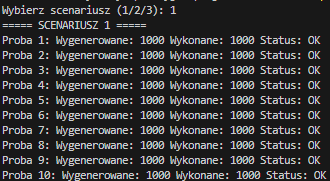
\includegraphics[width=0.95\textwidth]{scenariusz1.png}
                \caption{Scenariusz 1 - wynik w konsoli (kolejne próby i raporty końcowe).}
                \label{fig:scenariusz1}
            \end{figure}
        \newpage
        \vspace*{2em}
        \subsection{Scenariusz 2: test obsługi priorytetów}
            \vspace{-0.2em}
            Wynik pomiaru stanowią logi z wykonania, w tym informacja o dodaniu zadania HIGH do kolejki oraz dalsze logi przetwarzania zadań.
            \begin{figure}[H]
                \centering
                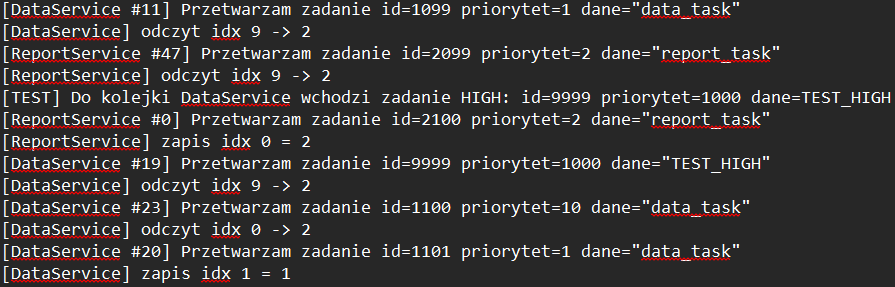
\includegraphics[width=0.95\textwidth]{scenariusz2.png}
                \caption{Scenariusz 2 - wynik w konsoli (log dodania zadania HIGH i przebieg przetwarzania).}
                \label{fig:scenariusz2}
            \end{figure}
            \vspace{1em}
        \subsection{Scenariusz 3: test procedury zamykania}
            \vspace{-0.2em}
            Wynik pomiaru stanowią logi z wykonania, w tym komunikat informujący o zakończeniu przyjmowania nowych zadań wypisywany po dodaniu ostatnich zadań do kolejek. Dalsze logi pokazują przetwarzanie zadań znajdujących się już w kolejce oraz końcowy raport zgodności liczników.
            \begin{figure}[H]
                \centering
                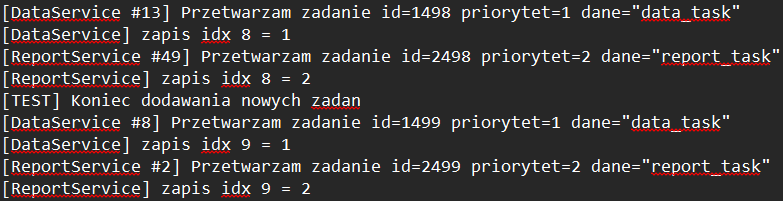
\includegraphics[width=0.95\textwidth]{scenariusz3.png}
                \caption{Scenariusz 3 - wynik w konsoli (komunikat oraz dokończenie pracy przez wątki).}
                \label{fig:scenariusz3}
            \end{figure}
    \newpage
    \vspace*{1em}
    \section{Wnioski}
        \vspace{0.5em}
        Na podstawie przeprowadzonych testów i obserwacji logów można sformułować następujące wnioski:
        \begin{itemize}
            \item Mechanizmy synchronizacji zastosowane w programie zapewniają spójność przetwarzania: we wszystkich zaprezentowanych uruchomieniach końcowe liczniki spełniają zależność Wygenerowane = Wykonane.
            \item Zastosowanie lokalnych kolejek priorytetowych w usługach pozwala sterować kolejnością pobierania zadań w obrębie danej usługi (zadania o wyższym priorytecie mają pierwszeństwo w kolejce).
            \item W scenariuszu 2 widoczny jest wpływ współbieżności i braku wywłaszczania: czasami pomiędzy logiem informującym o dodaniu zadania HIGH do kolejki a logiem jego przetworzenia pojawiają się logi innych, losowo wykonywanych zadań. Wynika to z tego, że priorytet porządkuje kolejność pobrania zadań z kolejki, ale nie przerywa zadania już wykonywanego oraz nie eliminuje przeplatania logów pochodzących z wielu wątków.
            \item Scenariusz 3 pokazuje rozdzielenie fazy generowania pracy od fazy przetwarzania: po informacji o zakończeniu przyjmowania nowych zadań wciąż pojawiają się logi przetwarzania, aż do całkowitego opróżnienia kolejki przez wątki robocze.
            \item Zamykanie programu jest realizowane w sposób łagodny: zatrzymanie polega na zamknięciu kolejki i dołączeniu wątków, co zapobiega utracie przyjętych zadań.
        \end{itemize}
    \newpage
    \vspace*{1em}
    \section{Podsumowanie}
        \vspace{0.5em}
        W ramach projektu zaimplementowano wielowątkowy serwer usług w języku C++, w którym każda usługa posiada własną kolejkę priorytetową zadań i pulę wątków roboczych. Zasoby współdzielone (logger oraz pula danych) zostały zabezpieczone odpowiednimi prymitywami synchronizacji, w tym modelem czytelnicy-pisarz dla danych globalnych. Przygotowane scenariusze testowe oraz zrzuty ekranu z uruchomień potwierdzają poprawność działania systemu, spójność liczników zadań oraz obserwowalny wpływ priorytetów i współbieżności na kolejność oraz przeplatanie logów.
        \vspace{1em}
    \section{Literatura}
        \vspace{0.5em}
        \begin{itemize}
            \item \href{https://pl.wikipedia.org/wiki/Wielow%C4%85tkowo%C5%9B%C4%87}{Wikipedia: Wielowątkowość}
            \item \href{https://en.wikipedia.org/wiki/Condition_variables}{Wikipedia: Condition variables}
            \item Dariusz Caban, Systemy operacyjne - prezentacje z wykładu (materiały dydaktyczne).
        \end{itemize}
    \newpage
    \vspace*{1em}
    \section{Kod}
        \vspace{0.5em}
        \subsection{main.cpp}
            \lstinputlisting{../main.cpp}
        \subsection{Task.hpp}
            \lstinputlisting{../Task.hpp}
        \subsection{SafePriorityQueue.hpp}
            \lstinputlisting{../SafePriorityQueue.hpp}
        \subsection{SharedResources.hpp}
            \lstinputlisting{../SharedResources.hpp}
        \subsection{Service.hpp}
            \lstinputlisting{../Service.hpp}
        \subsection{Service.cpp}
            \lstinputlisting{../Service.cpp}
\end{document}
